\chapter{A Replication Study on the Usage of Code Vocabulary to Predict Flaky Tests}
\label{chap:replication}

\setcounter{minitocdepth}{1}
\justifying
\textit{
In this chapter, we perform a replication of the vocabulary-based approach, one of the main techniques used to detect flaky tests. With this study, we intend to bring three contributions. First, we evaluate the approach under more realistic settings. Second, we check the generalisability of the approach by checking its application to another programming language. Finally, we experiment using an extended set of features in an attempt to improve the original approach.} \\

\chapterPage{This chapter is based on the work published in the following paper:\\
\begin{itemize}
\vspace{-2mm}
\item \fullcite{Haben2021}
\end{itemize}}

\section{Introduction}
\label{sec:replication-introduction}

Regression testing is an important step of software development that ensures the stability of existing software features and allow multiple developers to work on a shared codebase.  
In typical large-scale development workflows, test suites are run after code changes to highlight any misbehaviour and validate new software releases. 
Unfortunately, software tests do not always give consistent results. This inconsistent behaviour is often referred to as test flakiness. Flaky tests exhibit a non-deterministic nature, \ie they pass and fail for the same version of a program and the test~\cite{Luo2014}.

Flakiness plagues Continuous Integration (CI) as tests are generally expected to pass in order to merge code changes~\cite{CI}. Thus, flakiness introduces uncertainty, meaning that testers cannot be sure whether failures are true or not. 
Besides, flakiness affects productivity as developers invest time in reproducing and debugging flaky failures. 
Developers may also lose trust in their test suite and stop relying on it if there are too many false signals. 
Consequently, they could ignore failing tests that are caused by real defects in the program.

Several studies and reports from industrial actors have highlighted the prevalence and impact of flakiness~\cite{Lam2019RootCausing, LeongSPTM19, Kowalczyk2020}.  

A common approach to deal with flakiness is to rerun a failing test several times, hoping to expose non-deterministic behaviour. Unfortunately, these reruns imply cost both computationally- and time-wise. In the case of Google, this leads the company to spend between 2 and 16\% of its computer resources rerunning flaky tests~\cite{Micco2017}. Many other companies report having problems dealing with flaky tests, including Huawei~\cite{JiangHuawei}, Mozilla~\cite{Mozilla}, Facebook~\cite{Harman2018} and Spotify~\cite{FlakinessSpotify}.

To mitigate this problem, several strategies have been developed to detect flakiness. These can be divided into two main categories; the \textit{dynamic approaches} that involve running the tests and analysing their outputs and logs over time, and the \textit{static approaches} that attempt to identify flaky tests without any test execution. 

Micco and Memon~\cite{GTAC2016} presented a dynamic approach that identifies flaky tests by looking for specific patterns in the test execution outcomes observed in the recent development history (Pass to Fail, Fail to Pass), thereby proposing a simple pattern matching approach that achieves a 90\% accuracy in classifying tests~\cite{GTAC2016}. A similar approach was also presented by Apple~\cite{Kowalczyk2020}, but the reality is that rerunning tests is still the main dynamic approach used to detect flakiness~\cite{FlakinessGoogle}.

Pinto \etal~\cite{Pinto2020} developed a prediction modelling approach that statically identifies flaky tests by analysing their code (test code only). This approach is appealing compared to the current practice due to its static nature that a) does not require any test execution logging and analysis that is usually hard to implement on the fly and usually not supported by the test infrastructures, and b) the low overhead it entails, i.e., it reduces the execution cost caused by test reruns. 

The original study (Pinto \etal) evaluated the performance of different machine learning models on different representations of the test code and found that the vocabulary of tests can predict test flakiness with 95\% of accuracy (F1 score).
Although encouraging, the original study was performed in a dataset covering one programming language (Java), evaluated in a time-insensitive manner and left open many additional questions related to the vocabulary of source code. 
Considering the importance of the problem we decided to perform further investigations. We believe that extensive and independent evaluations are also necessary to reach industrial adoption and practice. 

Replication is essential to verify experimental results from previous studies. They are a key aspect of empirical software engineering as they bring evidence that observations made can hold (or not) under other conditions. Different types of replication exist~\cite{Shull2008,Gomez2014}. An \textit{exact} replication attempts to reproduce the experiments following as closely as possible the initial procedures. By doing so, we learn that the first results were not caused by uncontrolled random factors. In \textit{conceptual} replication, one or more dimensions can be changed to investigate to what extent the results hold. 

In this paper, we present a conceptual replication of the study of Pinto \etal~\cite{Pinto2020}.
We start by considering a different validation methodology than the one used in the study of Pinto \etal~\cite{Pinto2020}. We thus adopt a time-sensitive validation setting that better reflects the envisioned use case of the approach; at a given point in time, we train our predictor with historically identified flaky tests and inspect the model performance in predicting unseen flaky tests, i.e., with the subsequent ''future'' tests.  
We argue that this procedure is important to confirm the results and avoid biasing the predictions by considering future data. 

Another aspect our study aims to evaluate is the generalisation of Pinto \etal's findings, in particular to a different programming language. Therefore, we mine Python projects from GitHub and build a new dataset of 837 flaky tests. Then, we use it in order to evaluate the vocabulary-based flakiness prediction. This part of the analysis aims at re-validating the Pinto \etal findings on new and different data. 

Finally, we go beyond the original study by considering an extended set of features. In particular, we attempt to predict flakiness using not only the vocabulary of test code (like Pinto \etal did) but also the Code Under Test (CUT). This endeavour follows the findings of many reports\cite{Luo2014,Thorve2018,Lam2020b} revealing that much flakiness manifests in the CUT. Hence, we conduct a comparative study that highlights the impact of the two feature sets, \ie, sources of vocabulary on flakiness prediction.

All in all, our results demonstrate that a more robust, time-sensitive validation has a consistent negative impact on the reported results of the original study (performance degrades by 7\% on average) but, fortunately, do not invalidate the key conclusions of the study, \ie, predictions are significantly better than random selections. 

Additionally, we find re-assuring results that vocabulary-based models are more successful in Python than in Java (average performance of 80\% in Python in contrast to 61\% in Java), and perhaps surprisingly, that the information lying in the Code Under Test has a limited or no impact on the model performance. Taken together, these results corroborate the conclusion that the vocabulary of tests is indeed a viable and robust solution to the test flakiness problem.    

\section{The Original Study}
\label{sec:replication-pinto}

This work is a replication of the study by Pinto \etal \cite{Pinto2020}. 
In this section, we briefly summarise the approach they presented for flakiness prediction. 
We first present the dataset of existing flaky tests which they used in their study. Then, we explain their source code representation and prediction model. 
Finally, we recall their evaluation methodology and results. 

\subsection{Dataset}
In their original study, Pinto \etal relied on the DeFlaker dataset, which was proposed by Bell \etal~\cite{Bell2018}. 
This dataset includes 1,874 flaky tests identified using the DeFlaker tool on multiple revisions of 24 open-source Java projects.
Pinto \etal selected 1,403 flaky tests from this dataset to build their set of flaky tests.
They also randomly selected tests that were not flagged as flaky by DeFlaker to form a set of \textit{a priori} non-flaky tests. 
To mitigate the problem of class imbalance, both sets had the same size. 

\subsection{Prediction Model}
In order to prepare the classification inputs, Pinto \etal extracted identifiers that represent the test vocabulary and complexity. 
This extraction takes several steps. First, they localise the file where the test is defined. Then, they select all identifiers contained in this test, pre-process them by splitting them according to their camel-case syntax and converting them into lower-case. Finally, they remove stop words from the obtained set. Each flaky and non-flaky test is represented as follows:
\begin{itemize}
    \item A vector of booleans indicating for each token if it is present in the test or not;
    \item The number of lines of code;
    \item The number of Java keywords contained in the test.
\end{itemize}  
The last two features are used as a proxy for code complexity.
The authors used these vectors as inputs for their prediction models.
In particular, they evaluated the performance of five machine learning classifiers: Random Forest, Decision Tree, Naive Bayes, Support Vector Machine, and Nearest Neighbour. 
\subsection{Evaluation}
\subsubsection{Evaluation methodology}
The authors follow a standard methodology to train and evaluate the five classifiers. That is, they split the whole set of test cases into a training set containing 80\% of the tests and a validation (``test'') set containing the remaining 20\%.

\begin{table*}[t]
\vspace{1.0em}
\centering
    \caption{Model performance of the Pinto \etal study~\cite{Pinto2020}}
\label{table:resultsPinto}
\resizebox{\textwidth}{!}{\begin{tabular}{l l|r r r r r r} 
 \toprule
  & \textbf{Algorithm ~~~~~~~~~~~~} & \textbf{~~~~~~ Precision} & \textbf{~~~~~~ Recall} & \textbf{~~~~~~ F1} & \textbf{~~~~~~ MCC} & \textbf{~~~~~~ AUC} & \\ %[0.25ex]
 \midrule
  & Random Forest & \textbf{0.99} & 0.91 & \textbf{0.95} & \textbf{0.90} & \textbf{0.98}  &  \\
  & Decision Tree & 0.89 & 0.88 & 0.89 & 0.77 & 0.91  &  \\
  & Naive Bayes & 0.93 & 0.80 & 0.86 & 0.74 & 0.93  &  \\ 
  & Support Vector & 0.93 & \textbf{0.92} & 0.93 & 0.85 & 0.93  &  \\
  & Nearest Neighbour & 0.97 & 0.88 & 0.92 & 0.85 & 0.93  &  \\
 \bottomrule
\end{tabular}}
\vspace{1.0em}
\end{table*}

They report the standard precision, recall and F1-score metrics. The precision shows the proportion of correctly classified flaky tests. The recall shows the proportion of flaky tests found out of all existing ones. 
They focus their analysis on the F1-score, which combines precision and recall to assess the model performance. Detailed results for their different models are listed in Table ~\ref{table:resultsPinto}.

\subsubsection{Results}
Among the five trained models, the most promising one was Random Forest, having a performance as high as 0.95 for the F1-score. Altogether, the five models showed great performance on their dataset.  

\section{The Replication Study}
\label{sec:replication-replication}

Our key goal is to investigate whether the conclusions of Pinto \etal generalize to different flakiness scenarios, viz., (1) a time-sensitive prediction use case where flakiness information about past tests are used to predict flakiness in future (new) tests, (2) flakiness prediction in different programming languages, (3) the use of different sets of features involving both test code and code under test. Each of these scenarios gives rise to a research question that we answer in our study. In all scenarios, we use the model presented in the original study that gave the best performance. The model is based on a bag of words and a Random Forest of 100 trees i.e., the model which gave the best results in the original study. Our replication package containing code, models and datasets is available online\footnote{\url{https://github.com/serval-uni-lu/FlakyVocabularyReplication}}.

\subsection{Research Questions}
We aim at answering the following research questions:
\begin{itemize}[label={}]
\item \textbf{\textsc{RQ1:}} \emph{How  well  do  vocabulary-based  models  identify flaky  tests  when  using  a  time-sensitive validation?}
\item \textbf{\textsc{RQ2:}} \emph{How  well  do  vocabulary-based  models  identify flaky tests in other programming languages?}
\item \textbf{\textsc{RQ3:}} \emph{Is the vocabulary of Code Under Test useful for flakiness prediction?}
\end{itemize}

\subsection{RQ1: Time-Sensitive Validation}
In the real world, one can picture different usages for a flaky test prediction model. 
For instance, in Continuous Integration (CI) environments where new changes (commits) making some tests fail are typically rejected, developers can ignore those failing tests that are likely to be flaky and isolate them for further investigation.

In another setting, the prediction model can also come as an IDE plugin hinting at tests that use keywords related to flakiness.

These scenarios illustrate the importance of the temporality of tests and code, as the model can be trained only on flaky tests detected previously to predict new occurrences.
Moreover, the fact that the vocabulary of code changes as new commits are introduced makes it challenging for models trained on older data to predict flakiness in future code versions that are temporarily distant.

The model can also be limited to flaky tests detected in one project, e.g., when the vocabulary linked to flakiness can differ from one project to another. 
Indeed, as reported in the literature~\cite{Luo2014,Lam2019RootCausing}, different sources of flakiness exist such as concurrency issues, usage of date/time, I/O actions, API or network calls, etc. 
Thus, based on the project, the flakiness sources can differ and the vocabulary associated with it varies accordingly.

For all these reasons, we propose a novel, intra-project, time-sensitive setup for validating flakiness prediction models.
This setup evaluates a model on its ability to predict new flaky tests with data that is assumed to be known from the past of the project.

To compare this setup with the one from Pinto \etal, we rely on the DeFlaker dataset, which was also used in the original study.
For each project, we select tests that were found flaky at any revision of the change history to form the Flaky Tests set $FT$. 
DeFlaker does not provide explicit information about tests that did not flake, as the tool can not guarantee that a test that did not fail (yet) is not flaky. 
We define Non Flaky Tests $NFT$ as tests that were not found as flaky in any revision, that is, $NFT = T_{Total} - FT$.

Figure~\ref{time-validation} explains how FT and NFT are selected in our time-sensitive validation. We split our dataset in order to have 80\% of the FT from earlier revisions for our training set and 20\% of the FT from "future" revisions for our test set. 

We select the $NFT$ from the revision where the last $FT_{train}$ are selected for the training set and from the last revision where $FT_{test}$ are selected for the test set.

To assess the impact of this new setup on model performance, we compare it with a classical setup where the model is trained and tested with flaky tests regardless of their observation date (i.e., the setup followed by Pinto \etal).
In such setup, all flaky and non-flaky tests are grouped without accounting for their observation date. 
Then, the groups are randomly split into training and test sets following an 80/20 ratio. 

\begin{figure}
\centering
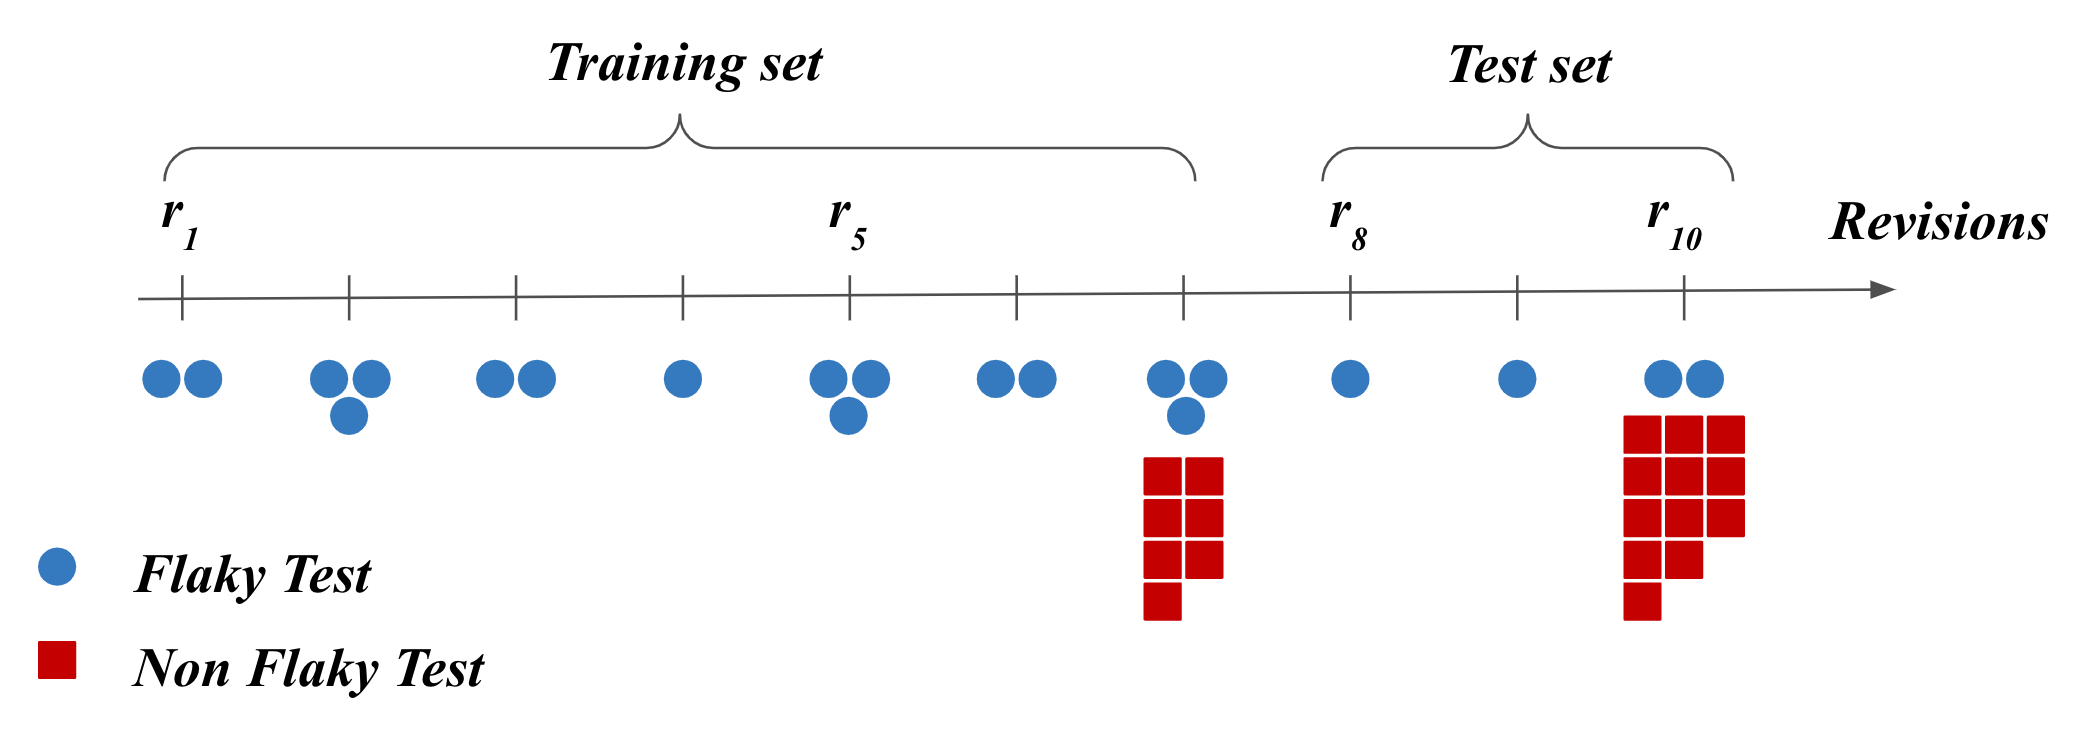
\includegraphics[width=0.8\textwidth]{figures/replication/fig1.png}
\caption{Time-sensitive validation}
\label{time-validation}
\end{figure}

To perform this comparison, we selected six projects from the DeFlaker dataset based on their numbers of flaky tests. 
These projects have at least 30 flaky tests, which we consider as a minimum necessary for training and testing a model. 
Table ~\ref{javaInfo} presents these projects with their numbers of flaky and non-flaky tests.
We also present the dates of the first and last flaky tests identified in these projects.
We split this dataset according to the two validation setups, then we build our prediction model, train it and contrast the results of both setups.

\begin{table}
\centering
\caption{Details about the Java projects used in our study}
\label{javaInfo}
 \begin{tabular}{l|r r r r r} 
 \toprule
 \textbf{Project} & \textbf{Earliest revision} & \textbf{Latest revision} &\textbf{ \#FT} & \textbf{\#NFT} \\ [0.25ex]
 \midrule
 achilles & 2015-10-30 & 2016-09-05 & 51 & 392 \\
 hbase & 2010-05-17 & 2010-06-21 & 98 & 120\\
 okhttp & 2014-03-06 & 2015-01-30 & 102 & 1178\\
 oozie & 2013-03-20 & 2013-05-31 & 1039 & 44 \\
 oryx & 2015-01-06 & 2015-02-27 & 38 & 286 \\ 
 togglz & 2016-01-23 & 2016-06-17 & 20 & 256 \\ 
 \bottomrule
\end{tabular}
\end{table}



\subsection{RQ2: Generalisation to other Programming Languages}
\subsubsection{Predicting flaky tests in Python}
Another goal of our study is to evaluate the generalisability of the original study to other programming languages.
For this purpose, we propose to assess the performance of flakiness prediction models on Python projects. 
We chose Python because it is the most popular language used in modern projects and it is commonly used for machine learning, web development, game development, and many other applications.

Python comes with its set of testing frameworks. 
We focus our study on Pytest\cite{pytestdocumentation}. Pytest is the equivalent of Junit for Python and enables developers to write tests for their programs. It is one of the main testing frameworks used in the open-source community and in the industry.
Pytest comes with its lot of features and plugins. Especially, a specific module to handle flaky tests can be used with Pytest: flaky\footnote{\url{https://pypi.org/project/flaky/}}.  
This module allows developers to annotate tests as flaky to automatically rerun them in case of failure. 
The developer can also configure the maximum amount of reruns to attempt and the minimum number of passes required. 
This annotation can be added to a test function or directly to the test class, giving its property to all of its tests. 
Figure~\ref{flaky-example} shows an example of a test marked as \emph{@flaky} taken from the Typed\_python project\footnote{\url{https://github.com/APrioriInvestments/typed\_python}}.

\begin{figure}[ht]
\centering
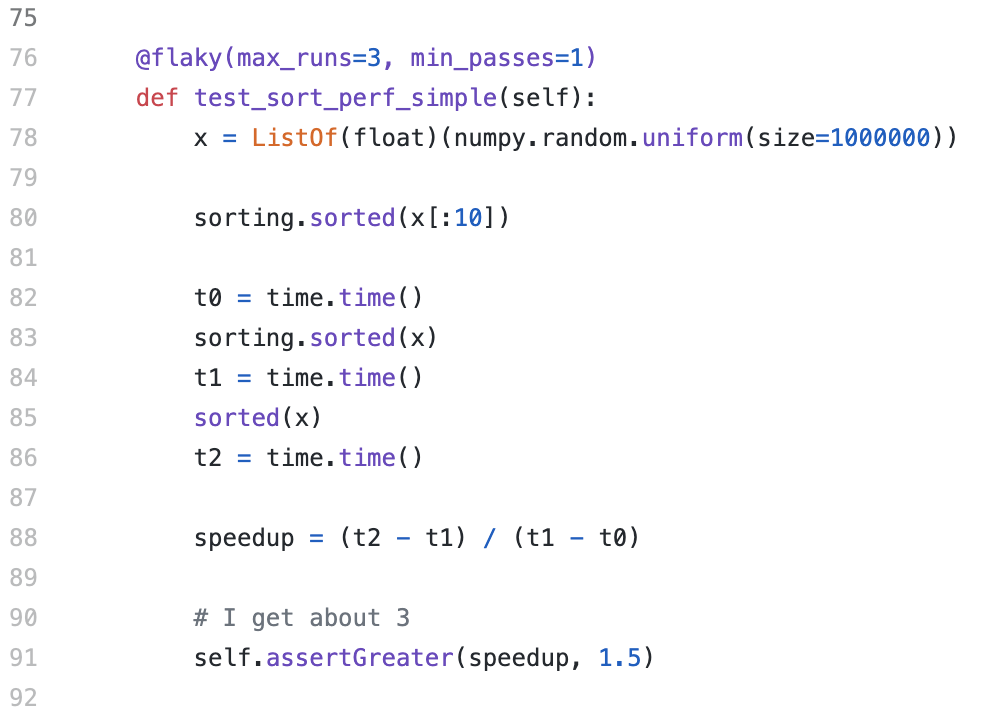
\includegraphics[width=0.8\textwidth]{figures/replication/flakyExample.png}
\caption{Example of a test labelled @flaky}
\label{flaky-example}
\end{figure}

We mined GitHub using the source-graph API\footnote{\url{https://sourcegraph.com/search}}, searching for Python projects containing the annotation \emph{@flaky}. 
This process yielded 110 projects with a total of 1,304 tests marked as flaky. 
Similarly to our first experimentation, we only select projects in which we have enough flaky tests to train and test a model, \ie 30 flaky tests.
This results in a dataset of 9 projects and 837 tests marked by developers as flaky.
Table ~\ref{pythonInfo} shows these projects with their number of flaky and non-flaky tests. 
Compared to the Java dataset, we were able to obtain more projects with more flaky tests for our study.
To the best of our knowledge, this is the first dataset of flaky tests in Python.

\begin{table}
\centering
\caption{Python projects used in our study}
\label{pythonInfo}
 \begin{tabular}{l|r r r r r} 
 \toprule
 \textbf{Project} & \textbf{SHA} & \textbf{\#FT }& \textbf{\#NFT}\\ [0.25ex]
 \midrule
 bokeh & ddc22b8 & 100 & 2505 \\
 cassandra-dtest & 8cb6bd2 & 72 & 4221 \\
 celery & 0833a27 & 54 & 2890 \\
 jira & 7fa3a45 & 131 & 59 \\
 pipenv & 8e64873 & 32 & 1612 \\
 python-amazon & 84c16f5 & 35 & 15 \\
 python-telegram-bot & 8e7c0d6 & 186 & 1382 \\
 spyder & 413c994 & 173 & 1086 \\
 typed-python & 96e7ebd & 54 & 6034 \\ 
 \bottomrule
\end{tabular}
\end{table}

It is worth noting that in this research question, we evaluate the performance of the model to predict flaky tests in a single revision. Therefore, we reuse the typical 80/20 dataset split as followed by Pinto \etal.  
That is, we are rather focusing on confirming that the approach works as well in Python and that a model can learn features differentiating tests labelled as \emph{@flaky} from the ones that are not. 
To extract these features, we use a bag of words representation of the test, as in Java. 
We also carefully remove the \emph{@flaky} annotations, as keeping it in the vocabulary would bias our model towards recognising this annotation rather than the code vocabulary.


\subsubsection{Predicting manifest flaky tests}
We perform further analysis in Python to assess the usefulness of a vocabulary-based model. 
Our objective is to evaluate the ability of a model to identify \textit{manifest} flaky tests based on training with tests labelled as flaky by developers. 
We consider as manifest flaky, every test for which we are able to observe non-deterministic behaviour dynamically.
This means that the test fails and passes at least once after several reruns.
To identify these manifest flaky tests, we reran 200 to 300 times the test suite of the three projects Bokeh, Celery and Python-telegram-bot. 
We run the test suites on a Mac machine with a 2,4 GHz 8-Core i9 processor and 32Gb of RAM.
The results of these reruns are presented in the table ~\ref{manifestStudy}.
The column \#@flaky shows the number of tests labelled as flaky in each project.
\begin{table}
\centering
\caption{Classifier performance for Python projects with manifest flaky tests}
\label{manifestStudy}
 \begin{tabular}{l|r r r r r} 
 \toprule
 \textbf{Project} & \textbf{\#reruns} & \textbf{\#@flaky} & \textbf{\#manifest FT}\\ [0.25ex]
 \midrule
 bokeh & 200 & 100 & 1 \\
 celery & 300 & 54 & 2 \\
 python-telegram-bot & 300 & 186 & 20 \\ 
 \bottomrule
\end{tabular}
\end{table}

We observe that despite the high number of reruns (800), only 23 tests have a flaky behaviour. This outcome is not surprising as flaky tests are, by nature, difficult to reproduce. To assess the model performance in detecting manifest flaky tests, we focus on the only project that has a reasonable amount of manifest flaky tests, namely Python-telegram-bot. We use the 20 manifest flaky tests found during our reruns as a test set, completed by 20 randomly selected tests that are not labelled as flaky. For the training set, we use the flaky and non-flaky tests minus the tests present in the test set. 

\subsection{RQ3: Extended Set of Features}
So far, the flakiness prediction is only based on features taken from the test code. 
However, flaky tests can be due to infrastructure or environmental issues (\eg lack of available resources in the CI, service or network unavailable, etc), to the test itself (\eg usage of dates, randomness, order dependency, etc), or to the CUT (\eg non-determinism, concurrency, etc). 
Notably, Luo~\etal~\cite{Luo2014} showed that 24\% of the fixes for flaky tests were applied to the CUT and that among them, 94\% fixed a bug in the CUT. 
Hence, it can be judicious to consider information from the CUT in flakiness prediction models. We propose to extend the original study by including the vocabulary of the CUT in test representation.

The main issue when considering the CUT is that computing the code coverage of each test during each revision would bring significant overheads. 
Besides, retrieving the exact code coverage dynamically goes against the goal of static prediction, which is to reduce dynamic costs.
To avoid this overhead, we propose a lightweight approach that relies on Information Retrieval (IR) to estimate the CUT. 

IR techniques have been used to solve different software engineering problems~\cite{Saha2014,Palomba2018,Azizi2018}. 
IR aims at quickly and automatically retrieving relevant information among a set of documents based on keywords taken from a user query. 
In our case, the query is the tokens of a test and the set of documents is the set of all functions (or methods) defined in the project. 
Our hypothesis is that functions from the CUT of a test are likely to use similar keywords (\ie variable names, API calls, etc) as the test. We are then looking for the most similar functions to our test function. To do so, we use a cosine similarity between a test case and a function from the CUT. Cosine similarity is defined with: 
\[cosSimilarity = \cos (Tc, Func) = \frac{Tc \cdot Func}{|Tc| |Func|}\]
where $Tc$ is the vector representing the test code and $Func$ is the vector representing the function code.
The result of a cosine similarity ranges from -1, meaning that the query - our test case - is completely different from the document - our function - to 1, where the query is perfectly similar to the document. 
In our case, we select the top three most similar functions for each test. 

\begin{algorithm}
\SetAlgoLined
\textbf{Inputs:}\\
Test[]\\
Function[]\\
\textbf{Outputs:}\\
TestWithCUT[]\\
\textbf{Procedure} \emph{CUT\_SELECTION(Test[], Function[])}\\
 \ForEach{ test T $ \in $ Test[]}{
   similarityMeasures[]\\
   Tvector = transform(T)\\
   \ForEach{function F $ \in $ Function[]}{
     fit($T+F$)\\
     Fvector = transform(F)\\
     cosTF = cosSimilarity(Tvector, Fvector)\\
     similarityMeasures.Append(cosTF)\\
   }
  similarityMeasures.Sort()\\
  similarityMeasures.Slice(0, 2)\\
  T.append(similarityMeasures)\\
  TestWithCUT.append(T)\\
 }
 \textbf{return} TestWithCUT[]
 \caption{Cost effective retrieval of the CUT}
 \label{algo}
\end{algorithm}

Algorithm~\ref{algo} describes the process of associating the CUT to each test. 
In order to compute the cosine similarity between the test and a function, we use the Text tokenisation utility class from the Keras library\footnote{\url{https://keras.io/api/preprocessing/text/}}. 
We first fit the \emph{Tokeniser} with the vocabulary from all tests and functions. 
Then, we transform the text of test and function bodies by creating a vector for each one of them of a length equal to the size of the vocabulary.
In this vector, each element represents the number of times a word appears in the body. 
After extracting the vectors, we compute the cosine similarity between the current test and all functions and store results. 
We finally filter to only keep functions that have a high score, \ie that they are the closest to the test. 
The body representation of the selected functions is used as a new set of features for the flakiness prediction model.
\section{Results}
\label{sec:replication-results}

\subsection{RQ1: Time-Sensitive Validation}

In this research question, we compare prediction model performance using a time-sensitive validation and a classical validation.

Figures~\ref{fig:prec-java}-\ref{fig:mcc-java} show the performance of our Random Forest classifier under time-sensitive and classical validation. 
Overall, we observe that the validation setup has an impact on the classifier performance.
This impact varies significantly depending on the project, its size, and history of flaky tests.
The projects Achilles, Hbase, OkHttp, and Togglz observe a decrease in their MCC score.
The largest performance drop is observed in the OkHttp project, where the MCC dropped from 0.39 to 0.18.
The two exceptions are for Oozie and Oryx, where MCC increased by 0.10 and 0.13 points respectively. 
In the case of Oryx, this can be explained by the fact that most of the flaky tests come from one revision, thus, the time-sensitive validation has little to no impact. 
The difference can then be explained by the random selection of the samples when splitting the training and test set. 
The phenomenon is only present for this project.
In the case of Oozie, there is a considerable imbalance between the number of flaky tests (1039) and non-flaky tests (44). 
Hence, the test set contains only 9 non-flaky tests, which might not be enough to draw conclusions.\\

\begin{tcolorbox}[
    left=2pt,right=2pt,top=2pt,bottom=2pt,
    arc=0pt,
    boxrule=1.2pt
]
\textbf{RQ1:} The performances of a vocabulary-based model decrease under a time-sensitive validation (MCC value drops up to 0.21).
Nonetheless, the approach is still able to decently predict flaky tests.
\end{tcolorbox}

\begin{figure}
  \centering
  \begin{minipage}[b]{0.4\textwidth}
    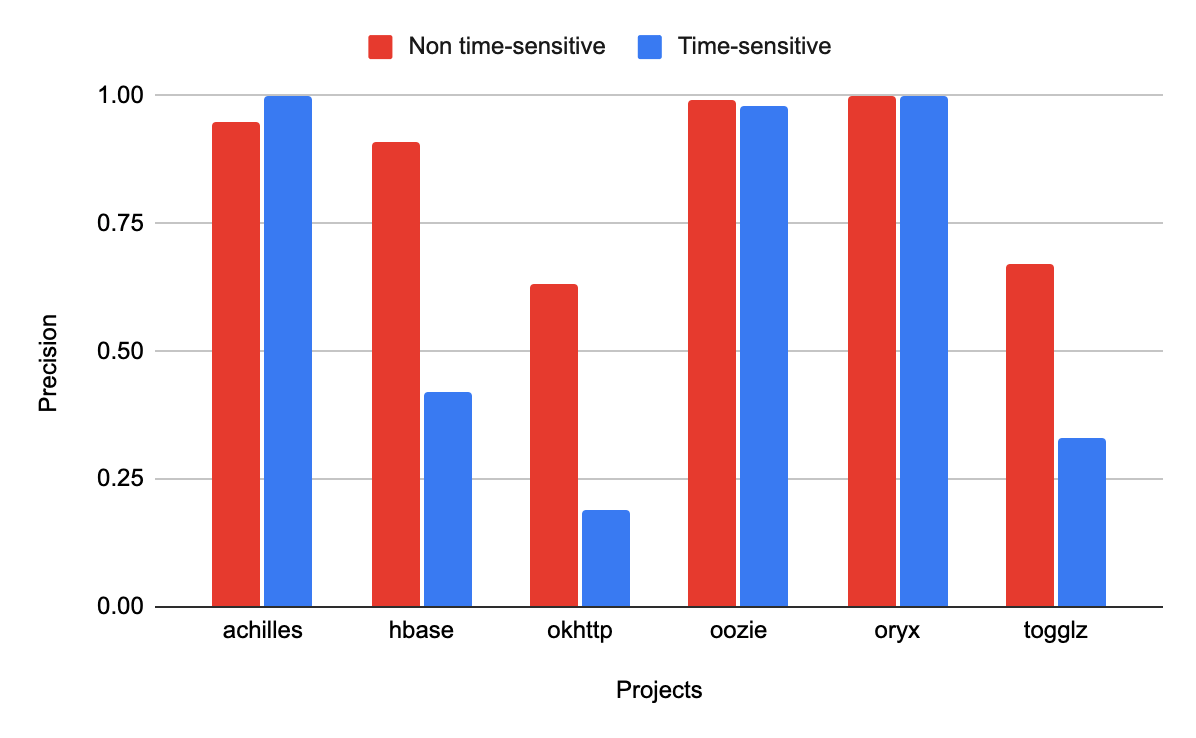
\includegraphics[width=\textwidth]{figures/replication/RQ1JavaPrecision.png}
    \caption{Precision under classical and time-sensitive validations.}
    \label{fig:prec-java}
  \end{minipage}
  \hfill
  \begin{minipage}[b]{0.4\textwidth}
    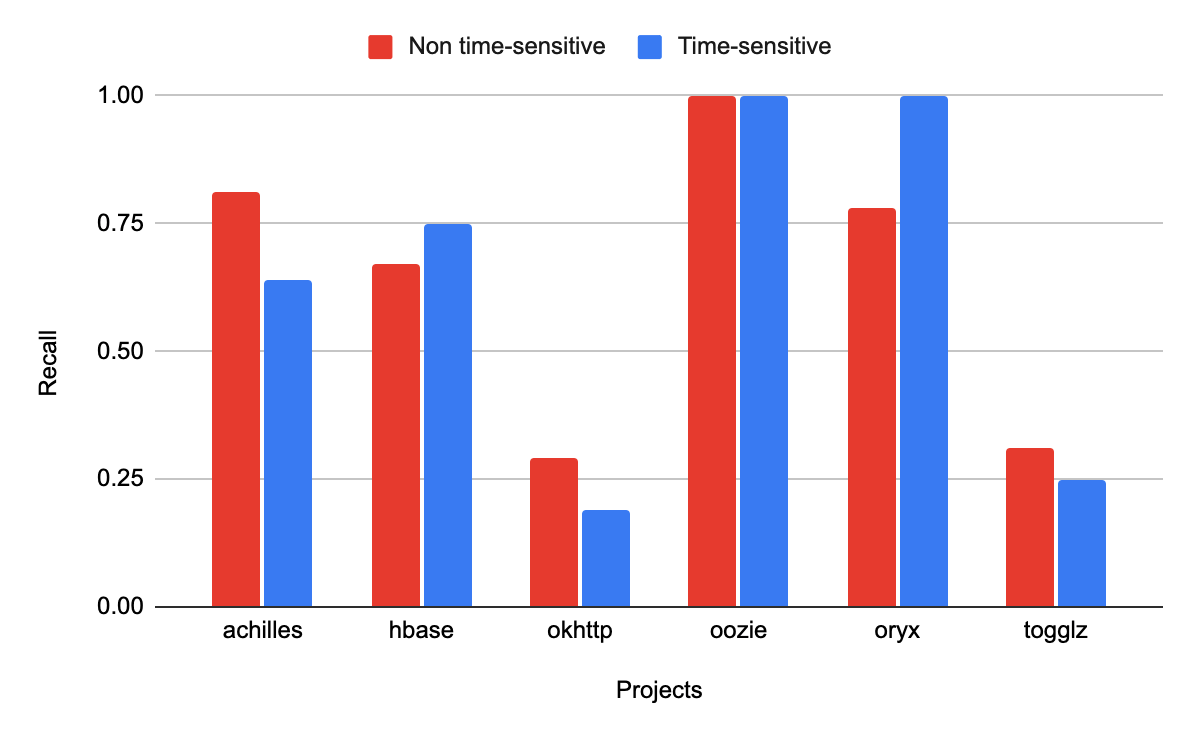
\includegraphics[width=\textwidth]{figures/replication/RQ1JavaRecall.png}
    \caption{Recall under classical and time-sensitive validations.}
    \label{fig:recall-java}
  \end{minipage}
  \hfill
  \begin{minipage}[b]{0.4\textwidth}
    \includegraphics[width=\textwidth]{figures/replication/RQ1JavaMcc.png}
    \caption{MCC under classical and time-sensitive validations.}
    \label{fig:mcc-java}
  \end{minipage}
\end{figure}

\subsection{RQ2: Generalisation to other Programming Languages}
\subsubsection{Predicting flaky tests in Python}
Table~\ref{python} reports on the model performance when predicting flaky tests in 9 Python projects. 

\begin{table}[t]
\centering
\caption{Classifier performance for Python projects}
\label{python}
 \begin{tabular}{l|r r r r r} 
 \toprule
 \textbf{Project} & \textbf{Precision} & \textbf{Recall} & \textbf{F1} & \textbf{MCC} & \textbf{AUC} \\ [0.25ex]
 \midrule
 bokeh & \textbf{1.00} & \textbf{0.91} & \textbf{0.95} & \textbf{0.95} & \textbf{0.95} \\
 cassandra-dtest & \textbf{0.96} & 0.43 & 0.58 & 0.63 & 0.71 \\
 celery & 0.85 & 0.54 & 0.64 & 0.66 & 0.77 \\
 jira & \textbf{0.98} & \textbf{0.99} & \textbf{0.99} & \textbf{0.95} & \textbf{0.98} \\
 pipenv & 0.78 & 0.19 & 0.30 & 0.37 & 0.60 \\ 
 python-amazon & \textbf{0.97} & \textbf{1.00} & \textbf{0.99} & \textbf{0.95} & \textbf{0.96} \\ 
 python-telegram-bot & \textbf{1.00} & \textbf{0.99} & \textbf{1.00} & \textbf{0.99} & \textbf{1.00} \\ 
 spyder & \textbf{0.92} & 0.77 & 0.83 & 0.82 & 0.88 \\ 
 typed-python & \textbf{1.00} & 0.86 & \textbf{0.91} & \textbf{0.92} & \textbf{0.93} \\ 
 \bottomrule
\end{tabular}
\end{table}

First, we observe that for 5 projects out of 9, the model reaches a great performance with MCC values greater than 0.9. 
For the rest of the projects, these scores are always higher than 0.50, except for Pipenv, which shows the lowest results with an MCC value of 0.37.
Similarly, all the studied projects have a F1-score greater than 90\% and 7 out of the 9 studied projects have a precision higher than 60\%.
These observations show that the vocabulary-based model is able to predict flaky tests with decent performance in Python projects.

\subsubsection{Predicting manifest flaky tests}

Table \ref{pythonManifestResults} shows the model performance in detecting manifest flaky tests based on tests marked as flaky by developers.
The results show a perfect performance with MCC and F1-score values of 1 and 100\% respectively, confirming that a model trained on tests labelled by developers can be used to predict manifest flaky tests.
Interestingly, 2 of the 20 manifest tests were not labelled as flaky by the developers and were only identified with the reruns.
Yet, the model was able to predict them by only learning from tests marked by developers.
In a real-world scenario, we could picture the model finding those tests and automatically annotating them.

\begin{table}[t!]
\caption{Classifier performance for manifest flaky test in the Python-telegram-bot project}
\label{pythonManifestResults}
\centering
 \begin{tabular}{l|r r r r r} 
 \toprule
 \textbf{Project} & \textbf{Precision} & \textbf{Recall} & \textbf{F1} & \textbf{MCC} & \textbf{AUC} \\ [0.25ex]
 \midrule
 python-telegram-bot & 1.00 & 1.00 & 1.00 & 1.00 & 1.00 \\ 
 \bottomrule
\end{tabular}
\end{table}

Figure \ref{manifest-flaky-example} shows the test \texttt{test\_idle()} from the class \texttt{TestUpdater}\footnote{https://github.com/python-telegram-bot/python-telegram-bot}.
Over 300 reruns, this test failed intermittently because of a concurrency issue where a scheduler has been shut down. 
Indeed, the test body contains several keywords related to time and concurrency, which are common causes of flakiness, \eg \texttt{Thread, sleep, idle}. 
In order to understand how the model predicted that this test is flaky, we analyse the most important features of the model. 
These features do not completely reflect the model prediction and they can be biased~\cite{Permutat82:online}, but they give us an idea of the vocabulary that the classifier is using for its predictions.
In the project Python-telegram-bot, we found that the top ten features include the keywords: \texttt{process, timeout, duration, seconds}, which are also related to time and concurrency.
Hence, the model's ability to predict the test flakiness based on the vocabulary.

\begin{figure}[ht]
\centering
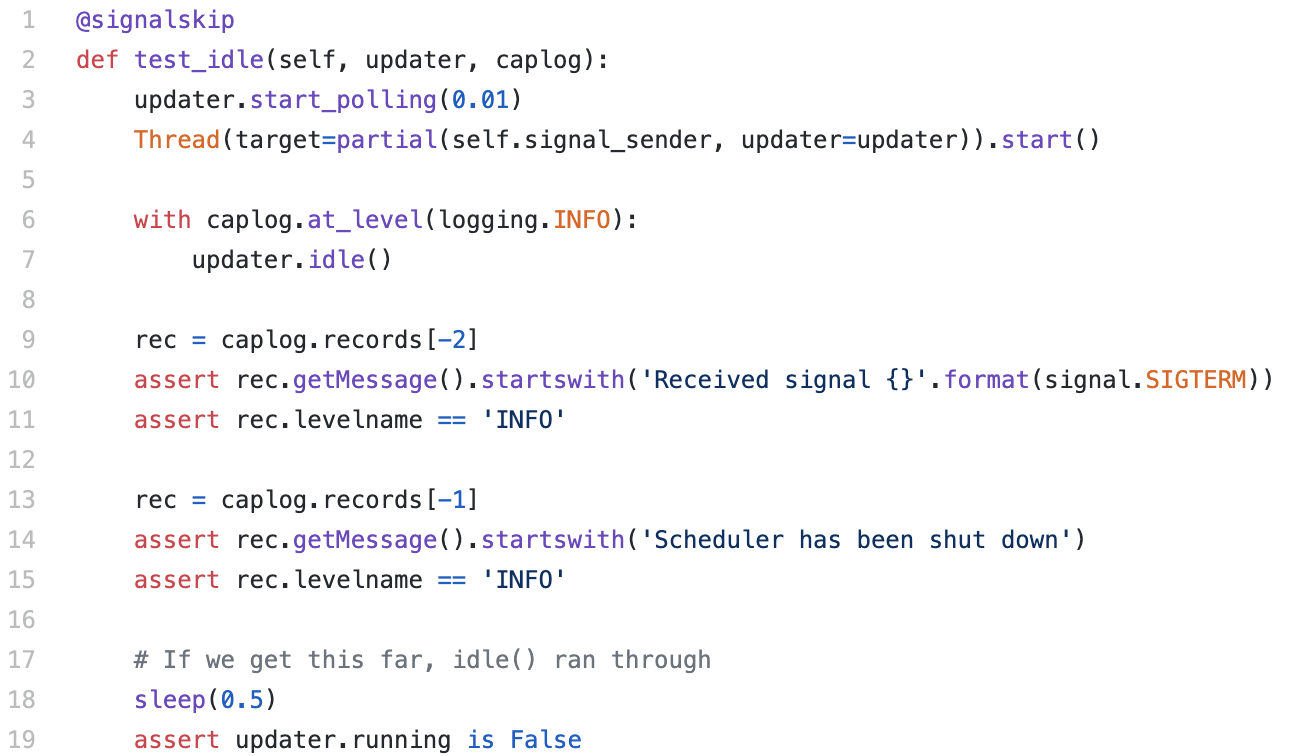
\includegraphics[width=0.8\textwidth]{figures/replication/manifestFlakyExample.png}
\caption{A manifest flaky test not labelled @flaky}
\label{manifest-flaky-example}
\end{figure}

Figure \ref{manifest-flaky-example2} shows the test \texttt{test\_to\_dict()} from the class \texttt{TestStickerSet}, which is also manifestly flaky but the developers did not mark it as such. 
Unordered collections have been identified as a cause of flakiness by several works as developers can wrongly assume that elements of a collection will be returned in a specific order~\cite{Luo2014,Dutta2020}.
In Python, the return order of dictionaries has varied over the different versions~\cite{PythonDoc, unorderedCollectionsStackOverflow}. In our case, we found that the keyword \texttt{dict}, which is present in a large number in this test, was among the first eight most important features of our classifier.
This feature allowed the vocabulary-based model to predict that this test is flaky.

\begin{figure}[ht]
\centering
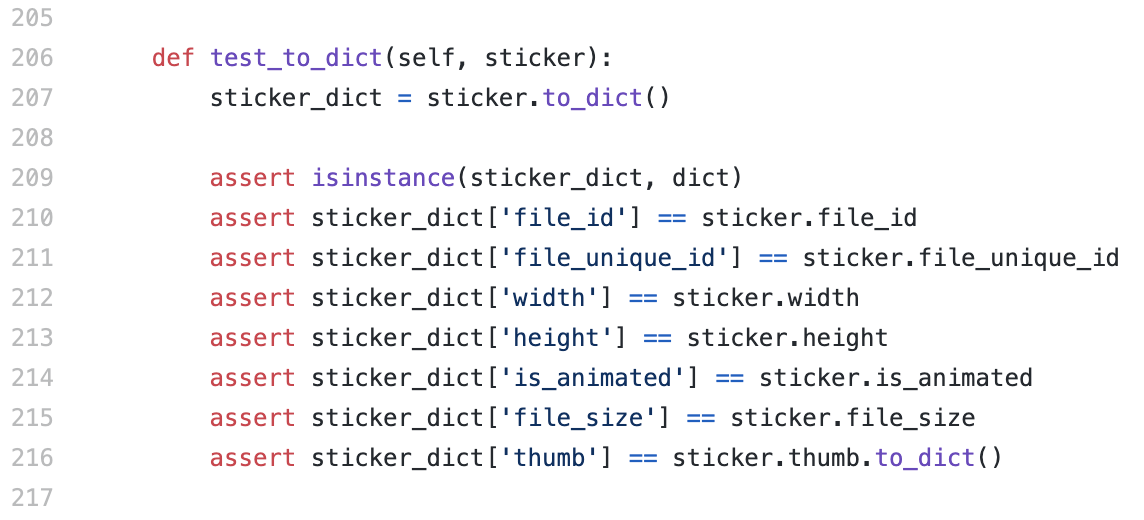
\includegraphics[width=0.8\textwidth]{figures/replication/manifestFlakyExample2.png}
\caption{A manifest flaky test not labelled @flaky}
\label{manifest-flaky-example2}
\end{figure}

We conclude that the approach is extendable to the Python language, supporting the idea that the vocabulary-based prediction can be generalisable to other projects and programming languages. Moreover, we saw that we can take advantage of a flaky tests classifier using vocabulary-based features in order to identify vocabulary linked to flakiness and help developers write better quality tests.\\

\begin{tcolorbox}[
    left=2pt,right=2pt,top=2pt,bottom=2pt,
    arc=0pt,
    boxrule=1.2pt
]
\textbf{RQ2:} Vocabulary-based models can be generalised to other projects and programming languages. 
Besides, these models can leverage annotated flaky tests to predict and annotate manifest flaky tests that were not known to developers.
\end{tcolorbox}

\subsection{RQ3: Extended Set of Features}

Figures~\ref{fig:prec-java-cut}-\ref{fig:mcc-java-cut} show the results of our prediction model in Java projects, while figures \ref{fig:prec-python-cut}-\ref{fig:mcc-python-cut} present the model performance in Python projects. 

\begin{figure}[!htbp]
  \centering
  \begin{minipage}[b]{0.4\textwidth}
    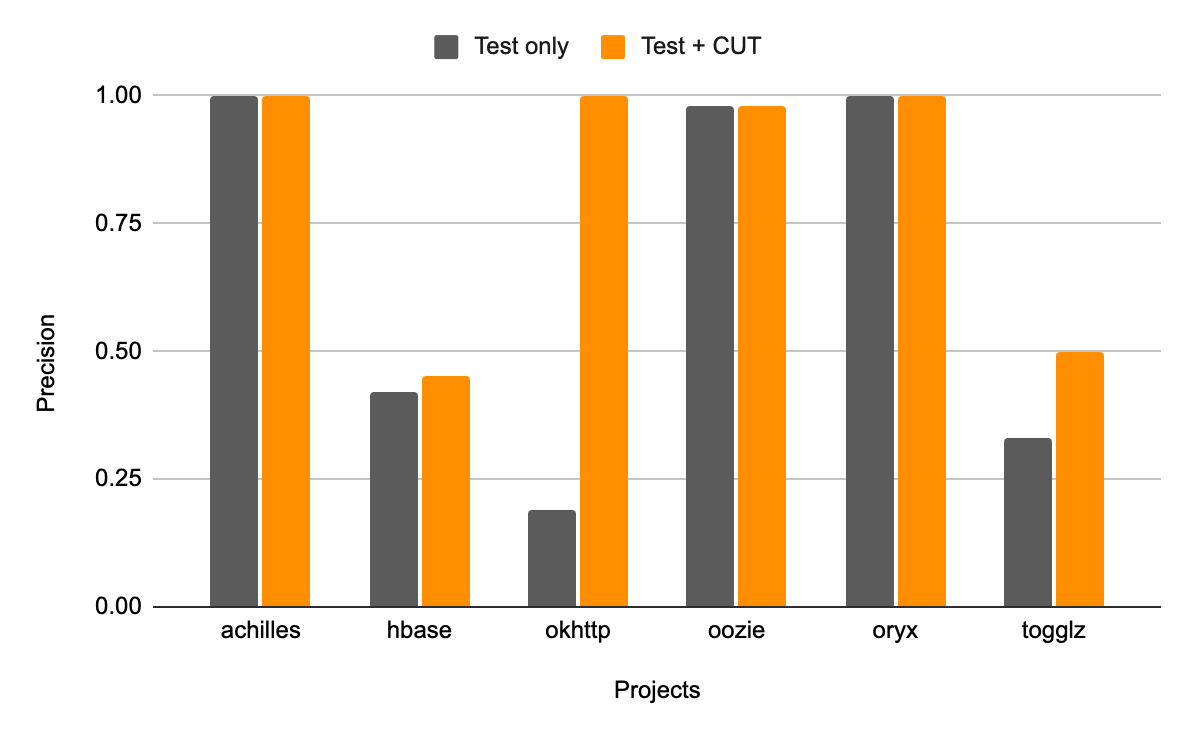
\includegraphics[width=\textwidth]{figures/replication/RQ3JavaPrecision.png}
    \caption{Precision score in Java projects}
    \label{fig:prec-java-cut}
  \end{minipage}
  \hfill
  \begin{minipage}[b]{0.4\textwidth}
    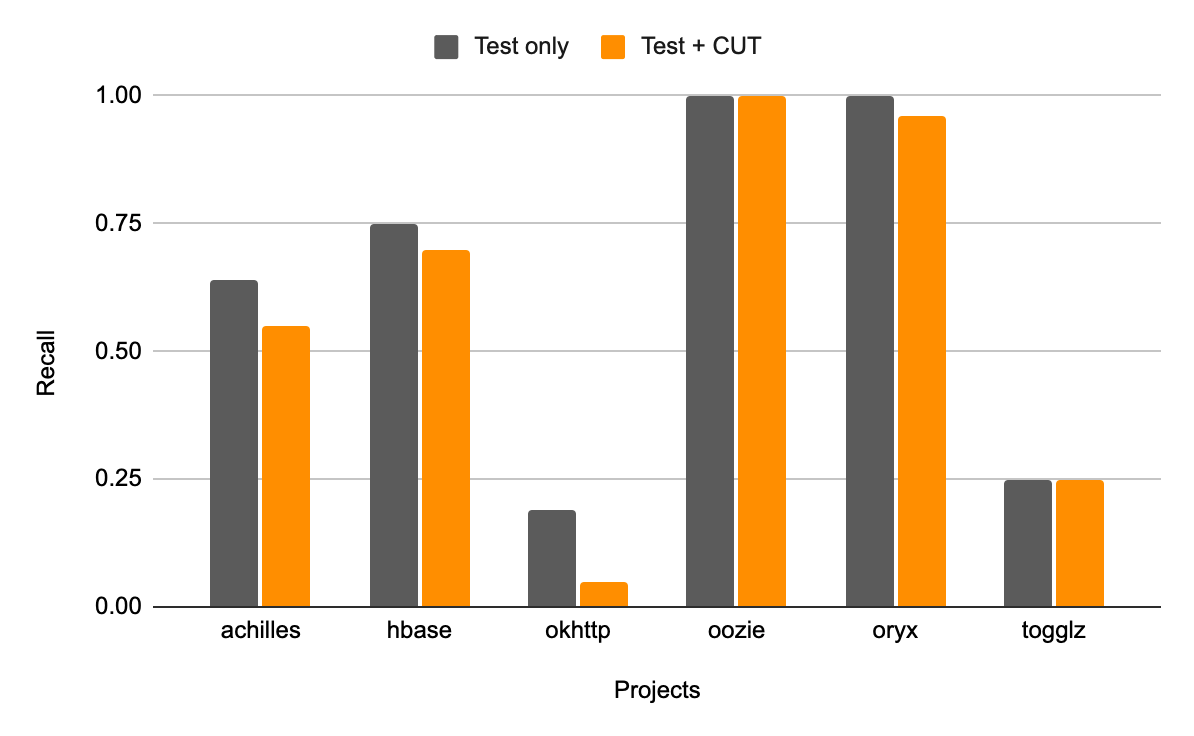
\includegraphics[width=\textwidth]{figures/replication/RQ3JavaRecall.png}
    \caption{Recall score in Java projects}
    \label{fig:recall-java-cut}
  \end{minipage}
  \hfill
  \begin{minipage}[b]{0.4\textwidth}
    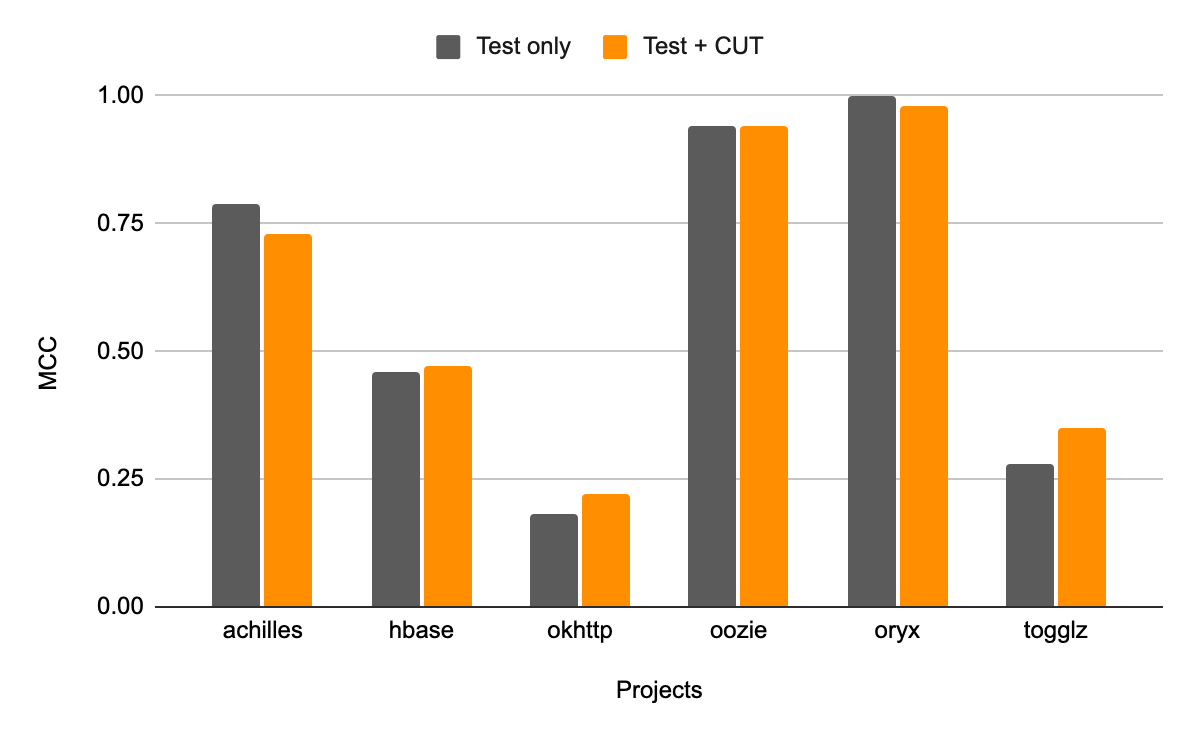
\includegraphics[width=\textwidth]{figures/replication/RQ3JavaMCC.png}
    \caption{MCC score in Java projects}
    \label{fig:mcc-java-cut}
  \end{minipage}
\end{figure}
\begin{figure}[!tbp]
  \centering
  \begin{minipage}[b]{0.4\textwidth}
    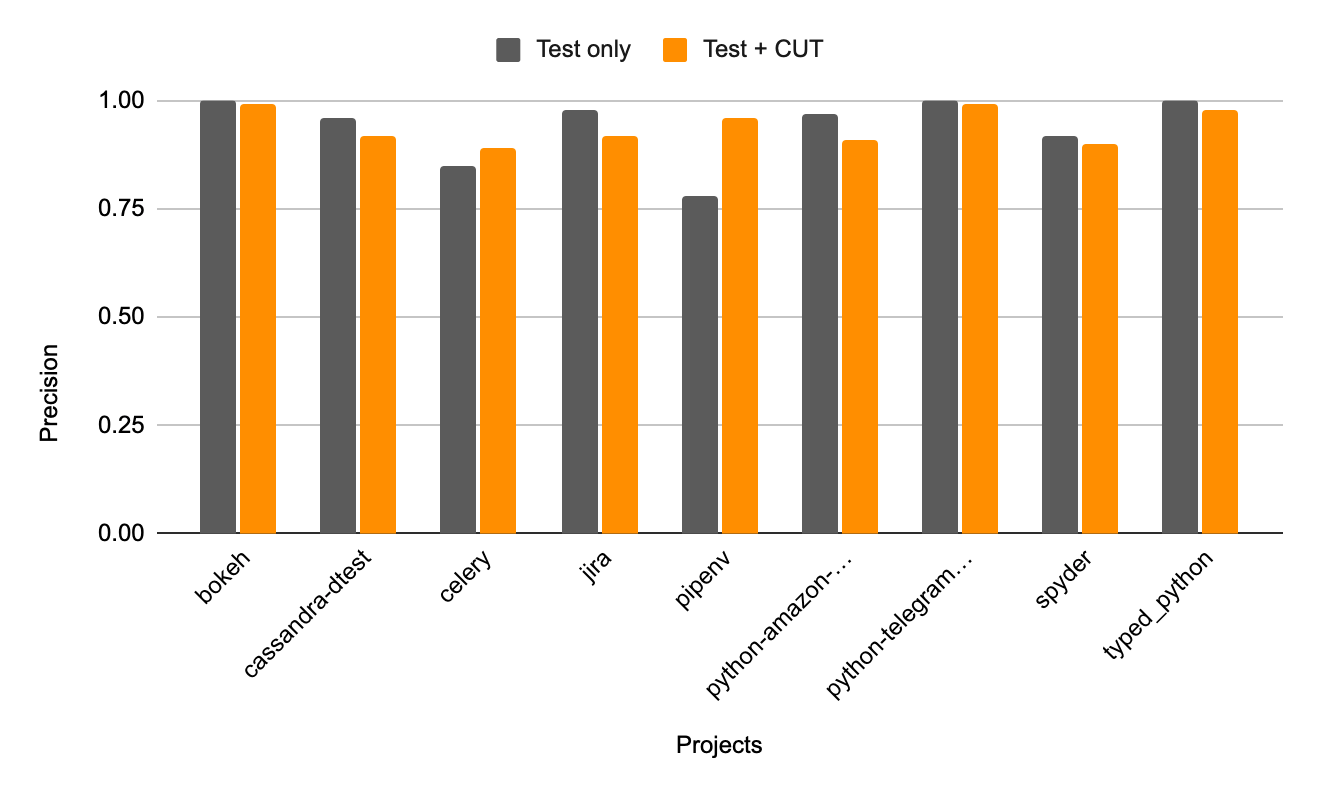
\includegraphics[width=\textwidth]{figures/replication/RQ3PythonPrecision.png}
    \caption{Precision score in Python projects}
    \label{fig:prec-python-cut}
  \end{minipage}
  \hfill
  \begin{minipage}[b]{0.4\textwidth}
    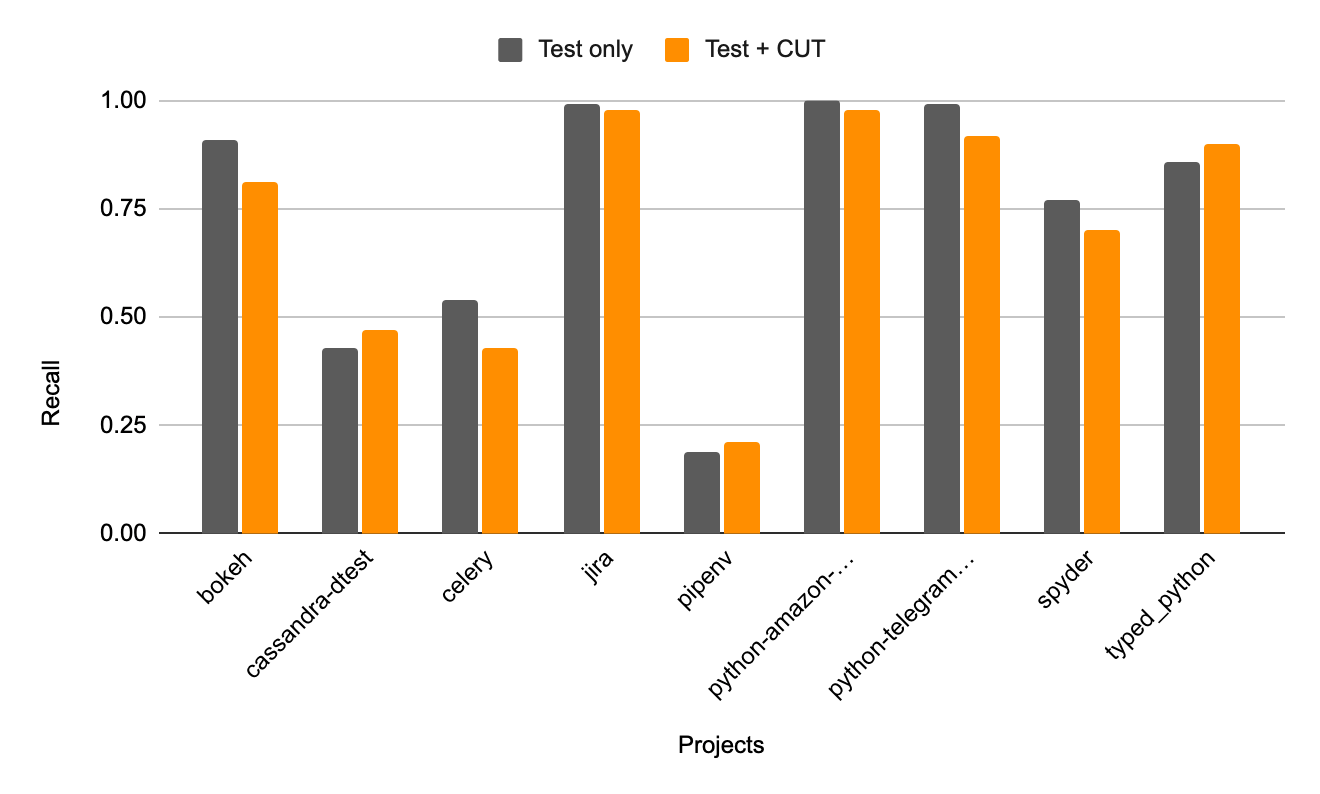
\includegraphics[width=\textwidth]{figures/replication/RQ3PythonRecall.png}
    \caption{Recall score in Python projects}
    \label{fig:rec-python-cut}
  \end{minipage}
  \hfill
  \begin{minipage}[b]{0.4\textwidth}
    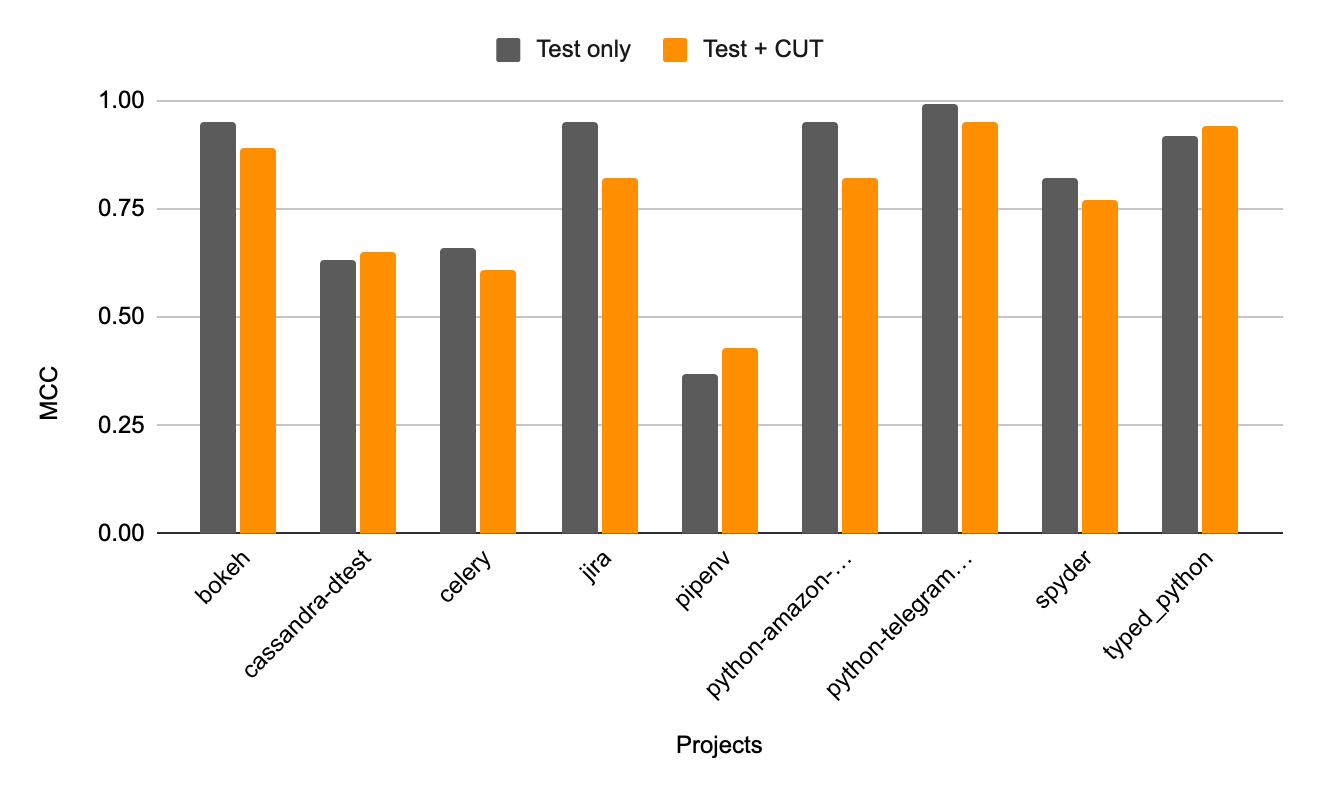
\includegraphics[width=\textwidth]{figures/replication/RQ3PythonMCC.png}
    \caption{MCC score in Python projects}
    \label{fig:mcc-python-cut}
  \end{minipage}
\end{figure}


In figures~\ref{fig:prec-java-cut}-\ref{fig:mcc-java-cut}, we observe that the impact of including the CUT does not have a consistent impact on the model performance in Java projects.
Adding the CUT improves the model performance in Hbase, Okhttp and Togglz, with an increase of the MCC value between 0.01 and 0.07.
However, the opposite effect is observed in the projects Achilles and Oryx where the MCC dropped by 0.06 and 0.02 respectively.
As for the Oozie project, including the CUT does not seem to impact the model performance.
Nonetheless, these performance improvements and losses remain minor in all the studied Java projects.

Figures \ref{fig:prec-python-cut}-\ref{fig:mcc-python-cut} show a similar effect of the CUT usage in Python projects.
Out of the nine studied, six projects report a lower performance when adding the CUT to the features.
This performance loss is up to 0.13 (MCC) in the projects Jira and Python-amazon.
On the other hand, the projects Cassandra-dtest, Pipenv, and Typed\_python have better predictions when the CUT is used --- an increase in the MCC value by 0.02, 0.06 and 0.02 respectively.

Based on the observations in both Java and Python, we conclude that including the CUT does not consistently improve the performance of a vocabulary-based model for predicting flaky tests.

\begin{tcolorbox}[
    left=2pt,right=2pt,top=2pt,bottom=2pt,
    arc=0pt,
    boxrule=1.2pt
]
\textbf{RQ3:} Surprisingly, the vocabulary of the Code Under Test, which is commonly considered as a source of flakiness, does not improve the performance of flakiness prediction models. 
\end{tcolorbox}

\section{Threats to validity}
\label{sec:replication-threats}







\subsection{Construct Validity}
One possible threat to the study's construct validity is our choice and selection of flaky tests in Python.
It is possible that tests that are marked as flaky by developers are not actually flaky.
In particular, developers could abuse of the annotation and mark non-flaky tests to forecast flaky behaviour.
To inspect this point, we manually analysed projects from our dataset to check if this behaviour is prevalent.
We found that some projects (like Jira and Python-telegram-bot) use the annotations to mark all class tests as flaky.
However, this usage seems judicious as the class tests performed GUI testing, which is known for being a major cause of flakiness.
Moreover, an abusive usage of this annotation by developers seems unlikely considering the rerun costs.
When running the test suites, we observed that one pass can take a long time.
Hence, it is not in the best interest of developers to mark as many tests as flaky to anticipate flakiness as this would largely increase the execution time as soon as there are test failures. 
We believe that the usage of annotated flaky tests in our study is reasonable given the lack of large datasets of flaky tests, especially for programming languages other than Java.
Ideally, the annotated flaky tests would be validated by rerunning them and exhibiting their non-deterministic behaviour.
Nevertheless, the reproduction remains very challenging for flaky tests in general and even tests identified in other datasets are hardly reproducible~\cite{Pinto2020,Lam2020}.
%Even with the DeFlaker dataset, which is, to our knowledge, the largest one existing to this date, most of the flaky tests are contained in one project (Oozie). It is difficult to find many flaky tests in one project, at least for open source projects that were studied. 

Another threat to construct validity could be our approach for retrieving the CUT. 
Intending to design a fast and lightweight approach, we used Information Retrieval to estimate the real code coverage of each test. 
This approximation can be responsible for the noise brought in the features. 
To investigate this point, we assessed the CUT effect when using other retrieval approaches. 
First, we retrieved an approximation of the CUT by using Static Call Graph. 
%Because the number of functions can easily explode when exploring the call graph, we stick to a depth level of 1: 
We selected all functions called by the test as the CUT and we do not explore what those functions call. 
Even if this approach only includes a subset of the CUT and flakiness can be caused by functions deeper in the call graph, we believe that keywords in the top functions should serve as proxy.
Results for this approach were similar to the ones presented in \textsc{RQ3}.
The performance scores slightly decrease or increase from one project to another without showing a significant impact on the prediction performance. 
Furthermore, we computed the code coverage for projects where we managed to build and run the test suite.
This task is challenging, especially in Java where the flaky revisions are from several years ago and dependencies are easily missing from central repositories. 
We successfully retrieved the real code coverage for revisions of Togglz and Oryx using the GZoltar tool~\cite{GZoltarA61:online}.
This tool allows us to get a coverage matrix representing each line covered by the test case. 
We used this matrix to retrieve the exact CUT and include it as a feature for our prediction model.
For both projects, the CUT inclusion had an impact on the model performance, which is very similar to the one observed with the CUT retrieved with IR.
Hence, we believe that the results observed in \textsc{RQ3} are not flawed by the CUT retrieval. 

\subsection{Internal Validity}
One possible threat to internal validity is the definition of non-flaky tests.
The datasets that we used for both Java and Python, only mark flaky tests and do not provide information about non-flaky tests.
Consequently, we considered all tests that were not marked as flaky to be non-flaky.
Yet, some of these tests can be flaky even though DeFlaker or the developer did not mark them as such.
This limitation is not unique to our study as it is theoretically impossible to prove that a test is not flaky.
To the best of our knowledge, there are no datasets, neither in formal nor in grey literature, that mark explicitly non-flaky tests.
On top of that, our study results show that there is a clear distinction between the classes of flaky and non-flaky tests.
Accordingly, it is unlikely that a significant fraction of the non-flaky tests is actually flaky.

One common threat to the internal validity of replication studies is potential errors in the reproduction (\eg settings and library usage). 
To alleviate this threat, we carefully examined the GitHub repository of the original work~\cite{damorimR19:online} to understand and reproduce their implementation details. 
%We tried to build our implementation as similar as possible. Still, we might not have used the same libraries or the same settings all the time, 
Besides, the goal of our study is not to exactly reproduce the original work and our results align well with the original findings.

\subsection{External Validity}
The main threat to our external validity is the size and nature of our datasets.
For Java, we relied on the DeFlaker dataset since it is the largest open-source set of flaky tests and it has already been used in many flakiness studies~\cite{Bertolino2020,Pinto2020}.
As for Python, we built a dataset of 837 flaky tests from 9 projects by mining GitHub repositories.
For the sake of generalisability, it would have been preferable to include more projects and flaky tests.
Nevertheless, our intra-project setting required a minimum number of flaky tests per project and limited our choices.
We encourage future studies to replicate this study on larger datasets, including industrial projects.




\section{Conclusion}
\label{sec:replication-conclusion}

% Flakiness is one of the main problems in Regression Testing. It easily increases the computational cost of Continuous Integration. Because it is hard to debug flaky tests, developers often spend a long time fixing them. In the worst case, they stop to consider flaky tests even if they could actually reveal a real defect in the program. To improve the efficiency of the CI and to strengthen the trust developers should have in their test suites, we must find ways to fight against this phenomenon. Prior studies tried to categorise and analyse flaky tests in order to get a better understanding of them. Recently, tools like DeFlaker or iDFlakies have been proposed to detect flaky tests. 

This paper explored the usability and performance of vocabulary-based models in predicting flaky tests. 
We presented a conceptual replication of the study of Pinto \etal, following three axes. 
\begin{itemize}
    \item First, we evaluated the prediction performances under a time-sensitive validation setting that better reflects the envisioned use case for the approach.
We found that a more robust validation has a consistent negative impact on the reported results of the original study (performance degrades by 7\% on average).
Fortunately, this performance degradation does not invalidate the key conclusions of the study as the model predictions are significantly better than random selections. 

    \item Second, we evaluated the generalisability of a vocabulary-based model to other programming languages. 
We found re-assuring results that vocabulary-based models are more successful in Python than in Java (average performance of 80\% in Python in contrast to 61\% in Java). We also showed that these models can leverage flaky tests annotated by developers to predict and annotate manifest flaky tests that were not known to developers.

    \item Third, we conducted a comparative study that highlights the impact of features lying in the CUT on the prediction performance.
    Surprisingly, we found that the vocabulary of the CUT, which is commonly considered as a source of flakiness, does not improve the performance of vocabulary-based models. 
\end{itemize}

%To do so, we presented our lightweight technique of retrieving the CUT with Information Retrieval. We compare results of our model for our Java and Python subjects, with and without the CUT and conclude that for those projects, and in the case of 
On top of these findings, this paper presents a new large dataset of flaky tests mined from developer annotations in Python projects on GitHub.
This dataset and our experiment toolset are available in a comprehensible replication package.

% We do that by building a dataset of 837 labelled flaky tests taken from 9 open-source projects available on GitHub.

% We believe that researchers should continue to explore ways of detecting flaky tests statically and proactively. For future works, we want to look for other approaches to reduce noise. One solution possible to explore is to switch from binary classification to multi-class classification by giving the information on the category of flakiness for each flaky test. This would require larger datasets, but could help to increase precision in our model and might also be used for fault localisation. 